%!TEX root = ../main.tex
%-------------------------------------------------------------------------------
%                            BAB II
%               KAJIAN TEORI
%-------------------------------------------------------------------------------

\chapter{Kajian Pustaka}

\section{\emph{Database}}

Pada Era teknologi saat ini, terdapat banyak sekali informasi-informasi 
yang tersebar. Mulai dari informasi mengenai pendidikan, penelitian, 
ekonomi dan lainnya. Informasi yang didapat bisa dikatakan sebagai data. 
Data dapat berbentuk angka, kumpulan kata, symbol dan lainnya. Data-data 
ini harus disimpan supaya bisa diolah atau disebarkan.  Untuk tercapai 
hal nya tersebut dibutuhkan sebuah teknologi untuk menyimpan data-data 
tersebut. Teknologi tersebut adalah \emph{database}. \emph{Database} adalah sebuah 
kumpulan data yang digunakan untuk mendukung aktivitas dari individu 
ataupun kelompok (\cite{databasedesignwatt}). \emph{Database} dapat berisi 
sebuah tabel, sebagai contoh sebuah \emph{database} perpustakaan dapat berisi 
tabel buku dan tabel pengunjung di mana kedua tabel tersebut dapat 
berkaitan satu sama lain. 

\emph{Database} juga dapat didefinisikan sebagai kumpulan data yang berkaitan 
di mana pengguna dapat mengambil data tersebut secara efisien 
(\cite{introductiondatabase}). Data-data yang telah dikumpulkan tersebut
sangat memungkinkan untuk diolah, diambil, dan diubah. Untuk melakukan 
hal tersebut dibutuhkan sebuah sistem yaitu \emph{database management 
system} yang disingkat sebagai DBMS. DBMS adalah sebuah program yang 
membuat pengguna dapat mengelola \emph{database} dan mengontrolnya 
(\cite{databasedesignwatt}). Tujuan utama dari DBMS adalah menyediakan 
aksesibilitas bagi pengguna agar dapat mengolah dan mengontrol 
data dengan baik. Di sisi lain DBMS juga harus untuk memastikan 
keamanan dari data yang telah disimpan dari pihak luar atau pihak 
tidak dikenal.

Berdasarkan buku \emph{database system}  (\cite{introductiondatabase}), DBMS merupakan manajemen data 
tersentralisasi. Terdapat beberapa kelebihan jika data disimpan secara tersentralisasi, kelebihan 
inilah yang juga menutupi kekurangan metode penyimpanan data sebelumnya yaitu \emph{file-based}. 
Berikut ini adalah beberapa kelebihan yang telah 
disebutkan pada buku tersebut (\cite{introductiondatabase}):

\begin{enumerate}
	\item Kontrol Redudansi Data \\
	\emph{Database} didesain untuk mengurangi redudansi data dikarenakan 
  sebagian besar data yang disimpan didalamnya terintegrasi 
  dengan data yang ada di tempat lain. Kondisi ini meminimalisir 
  terjadinya replikasi data pada tempat lain dan juga memastikan 
  konsistensi pada penyimpanannya. Walaupun dalam kondisi mungkin 
  saja  terjadi duplikasi data untuk mengoptimalkan performa saat 
  menggunakan \emph{database}.

	\item Integritas Data \\
  Pada penggunaan \emph{database}, penerapan integritas data menjadi 
  lebih mudah. Saat proses melakukan desain, pengguna dapat 
  menentukan hubungan dan relasi antar data pada \emph{database} yang 
  akan dibuat. Beberapa penerapan integritas data dapat dibuat 
  langsung di \emph{database} secara otomatis atau dapat melalui 
  aplikasi yang menggunakan data tersebut.

	\item Aksesibilitas \\
	Data yang disimpan di \emph{database} dapat diakses oleh beberapa 
  pengguna ataupun program. Dengan kasus seperti ini, bisa 
  saja terdapat dua aplikasi yang berbeda namun menggunakan 
  sumber data yang sama.

  \item Kemudahan dalam Pengembangan \\
  Dengan menggunakan DBMS, permasalahan seperti keamanan, 
  konkurensi, integritas data dan lainnya sudah ditangani 
  oleh DBMS itu sendiri. Pengembang aplikasi menjadi lebih 
  mudah karena tidak perlu memikirkan hal tersebut.

  
  \item Keamanan \\
  Karena penyimpanan data secara terpusat, membuat penerapan 
  keamanan menjadi lebih mudah. DBMS dapat memastikan bahwa 
  pengolahan data hanya bisa terjadi pada akses yang 
  diizinkan. Pada umumnya DBMS menyediakan sebuah code atau 
  password bagi pengguna yang ingin mengakses data.
\end{enumerate}


\section{Fitur-fitur pada \emph{Database}}
Berdasarkan buku \emph{database design} (\cite{databasedesignwatt}), \emph{database} (dalam pembahasan ini adalah \emph{relational database}) dapat memiliki banyak tabel. 
Setiap tabel tersebut juga dapat memiliki banyak kolom yang menyimpan data sesuai dengan kebutuhan dari pengguna. Setiap kolom yang ada di dalam tabel memiliki bisa memliki tipe data yang
berbeda-beda. Selain kolom, dalam \emph{database} memiliki baris data, dan nilai dari baris data tersebut akan berkaitan dengan kolom yang telah dibuat pada tabel. Tipe data dari baris juga harus
sama dengan tipe data dari kolom. 

Pengguna sering sekali membutuhkan akses kepada data yang telah tersimpan tersebut seperti melakukan pembuatan, pengambilan data untuk
melakukan analisa dan lainnya. Seperti yang dikutip pada subbab sebelumnya bahwa untuk melakukan pengolahan database, pengguna dapat menggunakan DBMS. Salah satu model DBMS yang
sering digunakan adalah \emph{relational} DBMS dan SQL (\emph{Structured Query Languange}) sebagai bahasa standar yang digunakan untuk mengakses DBMS. Berdasarkan buku \emph{database design} 
(\cite{databasedesignwatt}), SQL digunakan dalam DBMS untuk melakukan berbagai hal seperti:

\begin{enumerate}
	\item Membuat \emph{database} dan tabel

	\item Melakukan pengolahan data yang umum digunakan seperti (membuat, menghapus, dan mengubah)

  \item Melakukan pengambilan data untuk mengubah data mentah menjadi data yang dapat terbaca dengan baik
  
\end{enumerate}

Untuk melakukan pembuatan tabel, pembuatan \emph{database} harus terlebih dahulu dilakukan. Tabel akan memiliki sebuah nama, dan dalam tabel tersebut pengguna juga bisa membuat kolom yang banyak.
Kolom tersebut berisi nama dari kolom, tipe data dari kolom dan beberapa konfigurasi tambahan lainnya. Nama yang diberikan pada kolom harus bersifat unik dan tidak boleh sama antara satu
dengan yang lainnya. Untuk tipe data, SQL memiliki beberapa jenis tipe data yang didukung, beberapa di antaranya yaitu:

\begin{enumerate}
  \item Bit - Sebuah data integer bernilai 1 atau 0.

  \item Int - Data integer dari -2.147.483.6488 hingga 2.147.483.647

  \item Smallint - Data integer dari -32.768 hingga 32.767

  \item Tinyint - Data integer dari 0 hingga 255
  
  \item Uniqueidentifier - \emph{Global Unique Identifier} (\emph{GUID})
  
  \item Float - Tipe data yang mengambil data secara presisi

  \item Varchar - non-unicode karakter data yang berjumlah maksimal 8.000 karakter

  \item Text - non-unicode karakter data yang berjumlah maksimal 2.147.483.647 karakter
\end{enumerate}

Pada SQL, pengguna juga dapat menghapus kolom, menamnbahkan kolom, menghapus tabel dan beberapa
konfigurasi lainnya. SQL juga mendukung operator \emph{join} yang berguna untuk menghubungkan kedua tabel atau lebih. Pembahasan mengenai \emph{join} tabel akan dibahas pada subbab 2.6.

Di dalam DBMS umumnya juga memiliki fitur \emph{index} yang berguna untuk melakukan pengambilan data secara efisien. Berdasarkan buku
\emph{Database System} (\cite{databasesystem}), \emph{index} adalah sebuah struktur data yang disimpan dengan tujuan untuk mempercepat
akses terhadap sebuah data yang telah tersimpan. Pembahasan lebih rinci mengenai \emph{index} akan dibahas pada subbab 2.4.

\section{Arsitektur Internal \emph{Database Management System}}

Berdasarkan buku \emph{Database Internal} ({\cite{databaseinternal}}), 
arsitektur yang diterapkan dalam pengembangan \emph{database management system}, 
tidak mempunyai standar penerapan yang pasti. Setiap \emph{database} 
dapat dibuat dengan arsitektur yang berbeda dan arsitektur yang diterapkan pun juga 
sulit dilihat dan ditentukan. Meski arsitektur \emph{database}  ini dijelaskan pada sebuah tulisan seperti 
dokumentasi, dalam penerapan dan penulisan \emph{code} aslinya, arsitektur yang berbeda mungkin 
saja diterapkan untuk optimalisasi performa, penanganan beberapa kasus, atau 
keputusan arsitektur. Berikut ini adalah gambaran besar arsitektur 
DBMS yang sering digunakan.


\begin{figure}[H]
  \centering{}
	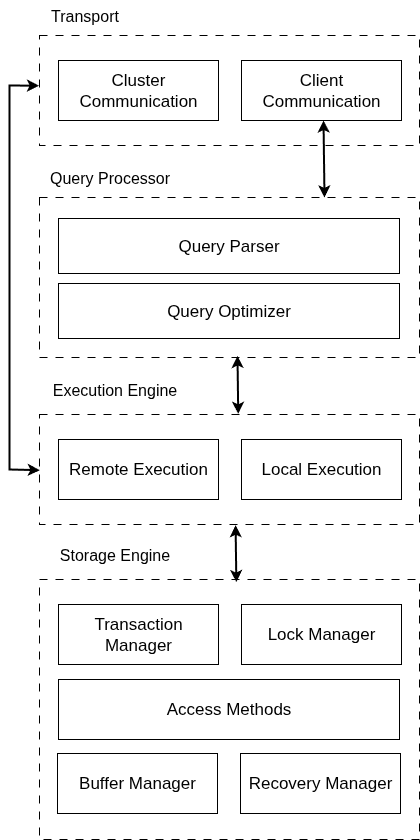
\includegraphics[width=0.5\textwidth]{gambar/bab2/dbms_achitecture}
  \caption{Ilustrasi Arsitektur \emph{Database}  Umum (\cite{databaseinternal})}
\end{figure}

\emph{Database management system} menggunakan \emph{client/server model}, di mana 
sebuah sistem \emph{database} berperan sebagai server, dan aplikasi mengambil 
peran sebagai \emph{client}. Permintaan \emph{client} akan diterima melalui 
\emph{transport subsystem}. Permintaan datang dalam bentuk sebuah \emph{query}, dan 
sering sekali dikatakan sebagai \emph{query language}. \emph{Transport subsystem} 
juga bertugas untuk melakukan komunikasi dengan node yang lain dalam 
cluster \emph{database} . Setelah menerima permintaan, \emph{transport subsystem} 
menyerahkan \emph{query} kepada \emph{query processor yang} akan menguraikan (\emph{parse}), 
menafsirkan (\emph{interprets}) dan melakukan validasi terhadap \emph{query} tersebut. 
Setelah semua proses ini selesai, pemeriksaan akses kontrol akan dilaksanakan.

\emph{Query} yang telah diuraikan akan diberikan kepada \emph{query optimizer}, yang 
akan menghilangkan bagian yang tidak memungkinkan untuk dijalankan dan bagian yang 
redundan dari \emph{query}. Lalu, sistem akan mencoba untuk mencari cara yang 
paling efisien untuk mengeksekusi \emph{query}-nya berdasarkan statistik \emph{internal} 
(kardinalitas \emph{index}, perkiraan ukuran \emph{intersection} dan lainnya) dan 
penempatan data (\emph{node} yang menyimpan data dalam \emph{cluster} dan biaya yang 
berkaitan dengan perpindahannya). \emph{Optimizer} menangani 2 hal yaitu, 
operasi yang dibutuhkan untuk resolusi pada \emph{query} (biasa dipresentasikan 
sebagai \emph{dependency tree}) dan optimisasi seperti pengurutan \emph{index}, estimasi 
kardinalitas dan pemilihan metode akses.

\emph{Query} biasanya dibuat dalam bentuk \emph{execution plan} (atau bisa disebut 
\emph{query plan}). \emph{Execution plan} adalah barisan / kumpulan operasi yang harus 
dibawa untuk memastikan hasil dianggap selesai. Karena \emph{query} yang sama 
dapat membuat hasil yang sama dengan \emph{execution plan} yang berbeda 
berdasarkan tingkatan efisiensinya, \emph{optimizer} akan mengambil \emph{execution 
plan} yang paling terbaik. \emph{Execution plan} akan diproses oleh \emph{execution 
engine} yang akan mengagregat hasil operasi dari lokal dan \emph{remote}. 
\emph{Remote execution} dapat meliputi proses writing (membuat, modifikasi, 
menghapus, dan lainnya) dan reading (mengakses) data dari node lainnya 
dalam cluster. \emph{Remote execution} juga dapat meliputi replikasi. 
Sementara \emph{local queries} (yang datang langsung dari \emph{client} atau \emph{node} 
lainnya) akan diproses oleh \emph{storage engine}. Sebuah \emph{Storage Engine} 
memiliki beberapa komponen yang masing-masing komponen tersebut memiliki 
tugasnya masing-masing, di antaranya adalah sebagai berikut:


\begin{enumerate}
	\item \emph{Transaction Manager} \\
	Komponen pengelolaan ini menjadwalkan \emph{transactions} dan 
  memastikan bahwa \emph{transactions} tidak dapat selesai dengan 
  kondisi \emph{state} didalamnya tidak konsisten.

		
	\item \emph{Lock manager} \\
	Komponen ini akan mengunci obyek \emph{database} untuk menjalankan 
  \emph{transactions}, untuk memastikan operasi konkurensi tidak 
  merusak integritas data.


	\item \emph{Access Methods} \\
	Komponen ini membantu pengelolaan akses dan mengorganisir 
  data dalam \emph{disk}. \emph{Access methods} meliputi \emph{heap files} dan 
  struktur penyimpanan seperti \emph{B-Trees} atau \emph{LSM Trees}.


  \item \emph{Buffer Manager} \\
  Komponen pengelolaan ini akan melakukan \emph{caching} data 
  halaman-halaman dalam \emph{memory}. 
  
  \item \emph{Recovery Manager} \\
  Komponen ini mengelola \emph{log} operasi dan merestorasikan 
  sistem jika sistem mengalami kegagalan.
  
\end{enumerate}
  
Secara bersama, \emph{transaction} dan \emph{lock managers} bertanggung 
jawab untuk pengendalian konkurensi. Keduanya menjamin 
integritas data logis dan fisik sambil memastikan bahwa 
operasi konkurensi dilaksanakan se efisien mungkin. Teori-teori yang dijabarkan diatas
ditulis berdasarkan informasi yang didapatkan dari buku (\cite{databaseinternal}).


\section{\emph{Database Index}}
Berdasarkan buku \emph{Introduction to Database System} (\cite{introductiondatabase}), setelah data berhasil disimpan
di \emph{disk} menggunakan metode-metode pengolahan \emph{file}, terdapat sebuah permasalahan utama yaitu bagaimana cara untuk
melakukan pengambilan data dengan cepat pada permintaan atau \emph{query} yang berbeda. Permasalahan ini dapat diselesaikan
dengan menggunakan sebuah struktur tambahan yang bernama \emph{index}. Sebuah \emph{file} dapat dibuat untuk menerapkan penamabahan stuktur 
\emph{index} ini. Penerapan \emph{index} tidak akan memengaruhi peletakan data yang telah disimpan sebelumnya, namun dapat memengaruhi kecepatan
dalam proses pengambilan datanya. Umumnya dalam suatu \emph{database}  dapat lebih dari 1.

Berdasarkan \emph{Pratical SQL, 2nd Edition} (\cite{praticalsql}), \emph{index} pada \emph{database}  berfungsi layaknya \emph{index} yang sering ditemukan pada buku. 
\emph{Query} dapat dipercepat dengan menambahkan sebuah \emph{index}, \emph{index} disini adalah sebuah struktur data terpisah yang dikelola
oleh sistem \emph{database}. Penerapan \emph{index} dalam \emph{database}  biasanya di terapkan pada kolom yang tersedia pada \emph{database}.
\emph{Database} akan menggunakan \emph{index} sebagai jalur cepat dalam melakukan pengambilan data daripada melakukan pengambilan data
dengan cara normal (melakukan pemindaian baris per baris).  

\section{Data Struktur \emph{Map}}

Berdasarkan buku \emph{Data Structures and Algorithms in Java, 6th Edition} (\cite{datastucturealgo}), Map adalah sebuah abstraksi data yang didesain untuk 
melakukan pengambilan dan penyimpanan data secara efektif. Map melakukan penyimpanan dan pengambilan data dengan mendefinisikan sebuah
\emph{key} yang bersifat unik untuk setiap nilai yang disimpan. \emph{Key} yang bersifat unik ini digunakan untuk melakukan pengambilan data
sehingga jika ingin mengambil sebuah data yang tersimpan maka harus mengetahui \emph{key} yang menjadi pasangan dari nilai tersebut.

Berdasarkan informasi dari buku \emph{A Common-Sense Guide to Data Structures and Algorithms, Second Edition, 2nd Edition} (\cite{commondatastucturealgo}), hampir semua bahasa
pemrograman memiliki fitur map ini. Hanya saja istilah yang digunakan pada masing-masing bahasa pemrograman berbeda-beda seperti \emph{Hash Table},
\emph{Hash Maps}, \emph{associative array} dan \emph{dictionary}. Walaupun istilah yang digunakan berbeda, namun yang tetap menjadi kelebihan adalah satu
yaitu kecepatan untuk pengambilan data. Untuk mencari sebuah value dalam struktur data map mempunyai tingkat efisiensi sekitar O(1) berdasarkan rata-rata.
Namun yang harus dijadikan catatan adalah untuk mencari value dalam map, pengguna harus mengetahui dulu key dari value tersebut. Jika tidak, maka pengguna harus
melakukan pengecekkan pada setiap \emph{key} dan \emph{value} dari \emph{map} tersebut. Hal ini menyebabkan tingkat efisiensi meningkat yang awalnya O(1) menjadi
O(N)

\section{Relasi antar Tabel (\emph{JOIN})}
Pada jenis-jenis \emph{database} , terdapat salah satu tipe \emph{database} yang sering digunakan yaitu \emph{Relational Database}. Berdasarkan buku 
\emph{Pratical SQL, 2nd edition} (\cite{praticalsql}), \emph{Relational Database} menyimpan data pada berbagai macam tabel yang saling berkaitan. Tabel yang saling berhubungan akan
menyimpan sebuah data tambahan yang bertujuan untuk menghubungkan tabel tersebut ke tabel lain. Untuk menggabungkan data antar tabel tersebut membutuhkan sebuah 
proses yang bernama \emph{join}. Pada \emph{relational database} seperti MySQL, terdapat beberapa metode dalam melakukan \emph{join} (\cite{praticalsql}), yaitu:
\begin{enumerate}
	\item \emph{JOIN} / \emph{INNER JOIN}\\
  Dengan menggunakan metode \emph{join} ini, data yang ditampilkan hanyalah data yang memiliki hubungan satu sama lain. Sehingga data yang tidak punya hubungan ke tabel lain, maka
  tidak akan ditampilkan.
  
	\item \emph{LEFT JOIN} \\
  Menampilkan seluruh baris data dari tabel sebelah kiri, dan ikut menampilkan data dari tabel sebelah kanan jika terdapat data tambahan pada tabel sebelah kiri yang memiliki
  hubungan ke tabel sebelah kanan.

	\item \emph{RIGHT JOIN} \\
  Prosesnya mirip dengan \emph{LEFT JOIN} akan tetapi berkebalikan. Menampilkan seluruh baris data dari tabel sebelah kanan, 
  dan ikut menampilkan data dari tabel sebelah kiri jika terdapat data tambahan pada tabel sebelah kanan yang memiliki
  hubungan ke tabel sebelah kiri.

	\item \emph{FULL OUTER JOIN} \\
  Menampilkan gabungan semua data dari tabel kiri dan tabel kanan. Akan tetapi jika dalam suatu baris terdapat data tambahan pada masing-masing tabel yang menghubungkan
  kedua tabel, maka baris dari kedua tabel tersebut akan bergabung menjadi satu. Untuk proses \emph{Full Outer Join}, jika dari masing-masing tabel tidak ada data tambahan yang
  menghubungkan antar tabel satu sama lain, maka proses \emph{join} ini tidak akan menampilkan apa-apa.

	\item \emph{CROSS JOIN} \\
  Menampilkan segala jenis kemungkinan penggabungan antar tabel tanpa memperhatikan data tambahan pada masing-masing tabel.

\end{enumerate}



\section{\emph{Database} Terdistribusi}

Berdasarkan buku \emph{database design}(\cite{databasedesignwatt}), dilihat dari jumlah penyebaran dan penggunaan sebuah \emph{database}, 
terdapat 2 cara penggunaan \emph{database} yaitu \emph{database} tersentralisasi 
dan \emph{database} terdistribusi. \emph{Database} tersentralisasi berjalan 
pada satu buah mesin. \emph{Database} dan DBMS berjalan pada sistem 
yang sama. Pengguna dapat berinteraksi dengan \emph{database} tersebut 
melalui koneksi yang telah terhubung pada mesin. Berikut 
adalah ilustrasi penerapan \emph{database} tersentralisasi:


\begin{figure}[H]
  \centering{}
	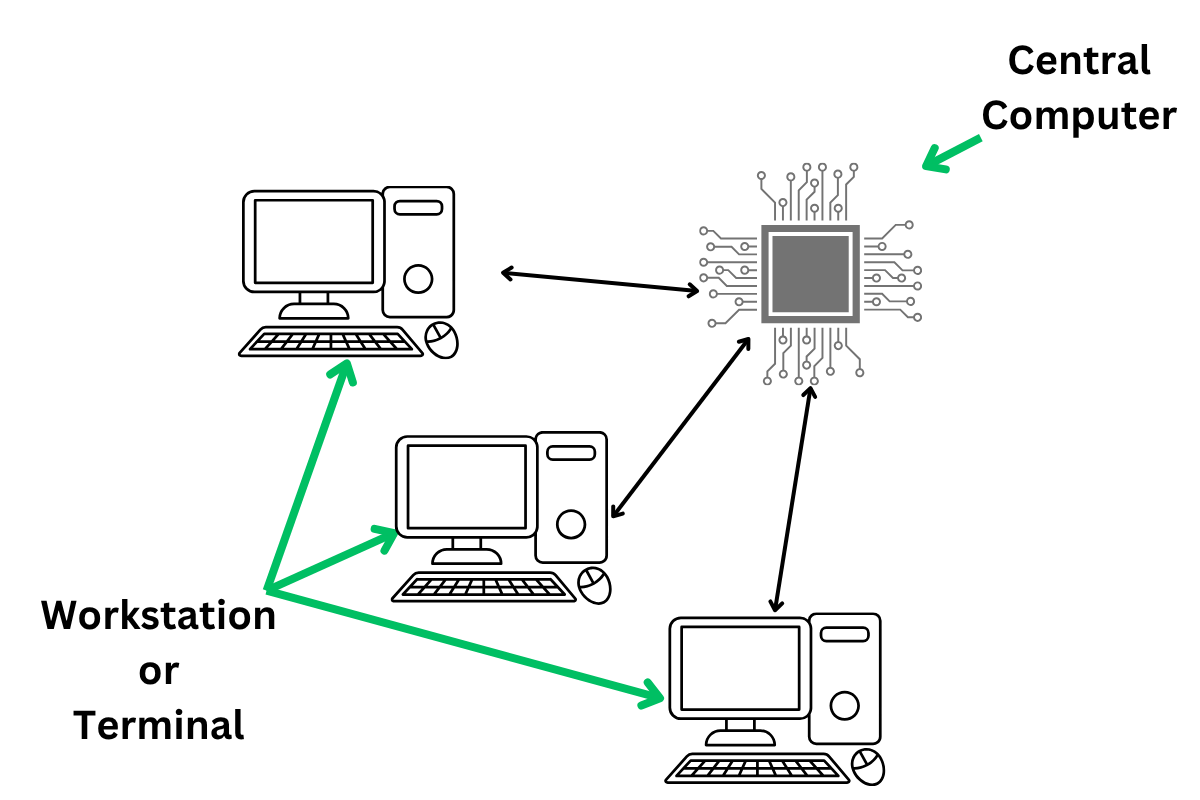
\includegraphics[width=0.65\textwidth]{gambar/bab2/centralized_db}
  \caption{Ilustrasi \emph{Database} Tersentralisasi (\cite{databasedesignwatt})}
\end{figure}

Sementara dalam \emph{database} terdistribusi, \emph{database} dan DBMS 
tersebar ke beberapa mesin yang berbeda. Antar mesin berkomunikasi 
satu sama lainnya melalui sebuah jaringan yang memiliki kecepatan 
tinggi. Berikut adalah ilustrasi dari penerapan \emph{database} terdistribusi:

\begin{figure}[H]
  \centering{}
	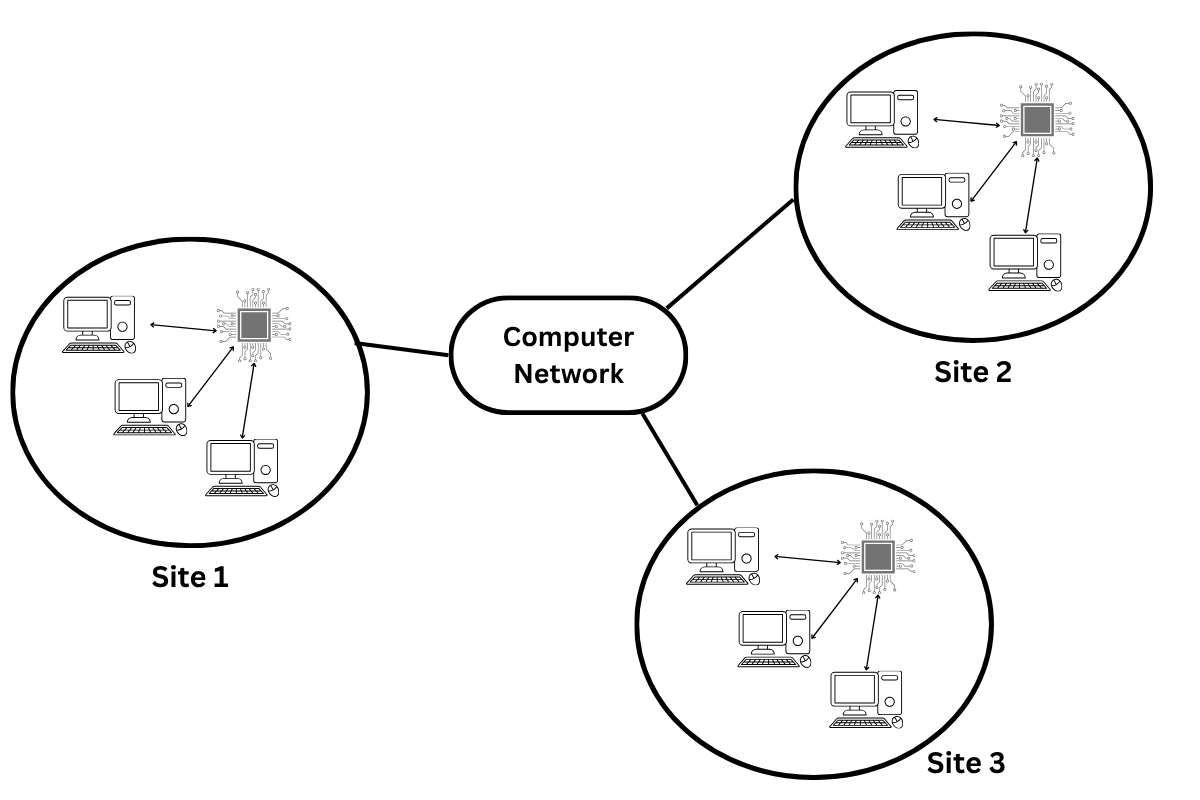
\includegraphics[width=0.65\textwidth]{gambar/bab2/distributed_db}
  \caption{Ilustrasi \emph{Database} Terdistribusi (\cite{databasedesignwatt})}
\end{figure}

\emph{Database} terdistribusi dapat diklasifikasikan menjadi 2 yaitu \emph{homogeneous} 
dan \emph{heterogenous}. \emph{Homogeneous} menggunakan DBMS yang sama antar mesin 
yang terhubung. Dengan begitu perpindahan dan pengolahan data antar mesin 
menjadi lebih mudah. Misalnya sebuah mesin A dan mesin B yang masing-masing 
didalamnya terdapat satu DBMS yang sama. Cara pengambilan data pada kedua 
mesin tersebut akan sama, sehingga ketika melakukan komunikasi, setiap 
mesin tidak perlu melakukan interpretasi kembali. Berikutnya terdapat 
\emph{heterogenous} yang pada penerapan \emph{database} terdistribusi, memungkinkan 
untuk memiliki DBMS yang berbeda antar mesin. Dengan penerapan ini, pengguna 
harus memastikan bahwa kedua DBMS yang berbeda tersebut harus bisa saling 
berkomunikasi. Salah satu penerapannya, beberapa \emph{database} menggunakan 
format \emph{machine-readable cataloguing} (MARC) yang sama untuk mendukung 
pertukaran data. 


\section{\emph{D-Bus}}
Berdasarkan dokumentasi dari freedesktop.org (\cite{dbus}), D-bus adalah 
sebuah \emph{message bus system}, sebuah cara sederhana untuk aplikasi 
berkomunikasi dengan aplikasi lainnya. D-Bus memiliki beberapa lapisan:

\begin{enumerate}
	\item \emph{libdbus} \\
  Merupakan sebuah \emph{library} yang berguna untuk menghubungkan kedua aplikasi satu sama lain dan bertukar \emph{messages}
  
	\item \emph{Message Bus Daemon Executable} \\
  Dibuat dengan libdbus, dan beberapa aplikasi dapat terhubung ke dalamnya. Daemon dapat menyalurkan \emph{messages} dari sebuah aplikasi ke beberapa aplikasi lainnya.

	\item \emph{Wrapper Libraries} atau \emph{Binding Based} \\
	\emph{Wrapper} yang digunakan berdasarkan \emph{framework} atau bahasa pemrograman yang digunakan. Contoh dari \emph{wrapper libraries} ini adalah
  \emph{libdbus-glib} dan \emph{libdbus-qt}. Masih terdapat hal lain seperti \emph{binding} dengan bahasa pemrograman. \emph{Wrapper libraries} ini digunakan untuk 
  mempermudah penggunaan D-bus. \emph{Library libdbus} sendiri memang ditujukan untuk melakukan \emph{binding} dengan \emph{higher level bindings}. Kebanyakan penggunaan API D-Bus
  dipergunakan untuk penerapan \emph{binding}.   
\end{enumerate}

\emph{libdbus} hanya mendukung koneksi \emph{one to one}. Paket pengiriman yang dikirim bukanlah \emph{bytes}, namun dikenal dengan istilah \emph{messages}.
\emph{Messages} mempunyai \emph{header} yang berguna untuk mengidentifikasi jenis dari \emph{message} nya, dan \emph{body messages} berisi sebuah data atau dikenal dengan
\emph{payload}. \emph{Library libdbus} juga akan menangani autentikasi. 

Untuk bagian \emph{message bus daemon}, berperan layaknya sebuah pusat pengiriman \emph{messages}. \emph{Bus Daemon} akan menerima \emph{messages} dari sebuah aplikasi
dan meneruskan \emph{messages} tersebut ke aplikasi yang dituju. \emph{Message bus daemon} dapat juga disebut sebagai \emph{router}. Umumnya pada setiap komputer memiliki
beberapa \emph{message bus daemon}. Berikut adalah diagram proses bekerja D-Bus.

\begin{figure}[H]
  \centering{}
	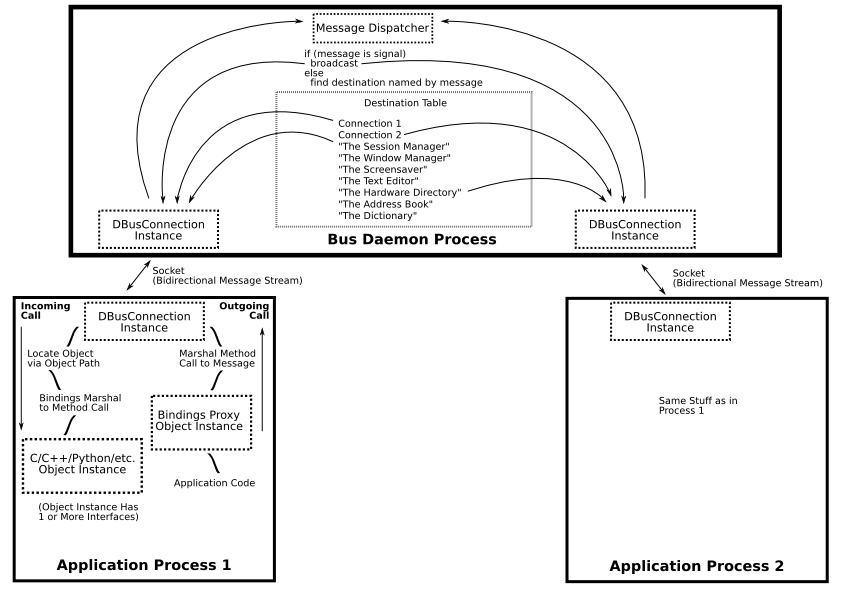
\includegraphics[width=0.95\textwidth]{gambar/bab2/dbus-architecure}
  \caption{Diagram alur D-Bus (\cite{dbus})} 
\end{figure}